\chapter{Rotationel Mekanik Udledning}
Her beskrives et fysisk pendul med masse $m$ og inertimoment $I$, hvor friktion ikke negligeres, og slutteligt vises det, hvad visse simplificeringer resulterer i. Det er tiltænkt at deltagerne selv laver kraftanalysen og beslutter hvilke kræfter, de antager pendulet er påvirket af, selvom snoren bør antages masseløs. Fremgangsmåden er den samme, så alle specialtilfælde beskrives ikke i detajler her. \\

\begin{figure}[]
\centering
\begin{subfigure}{.5\textwidth}
  \centering
  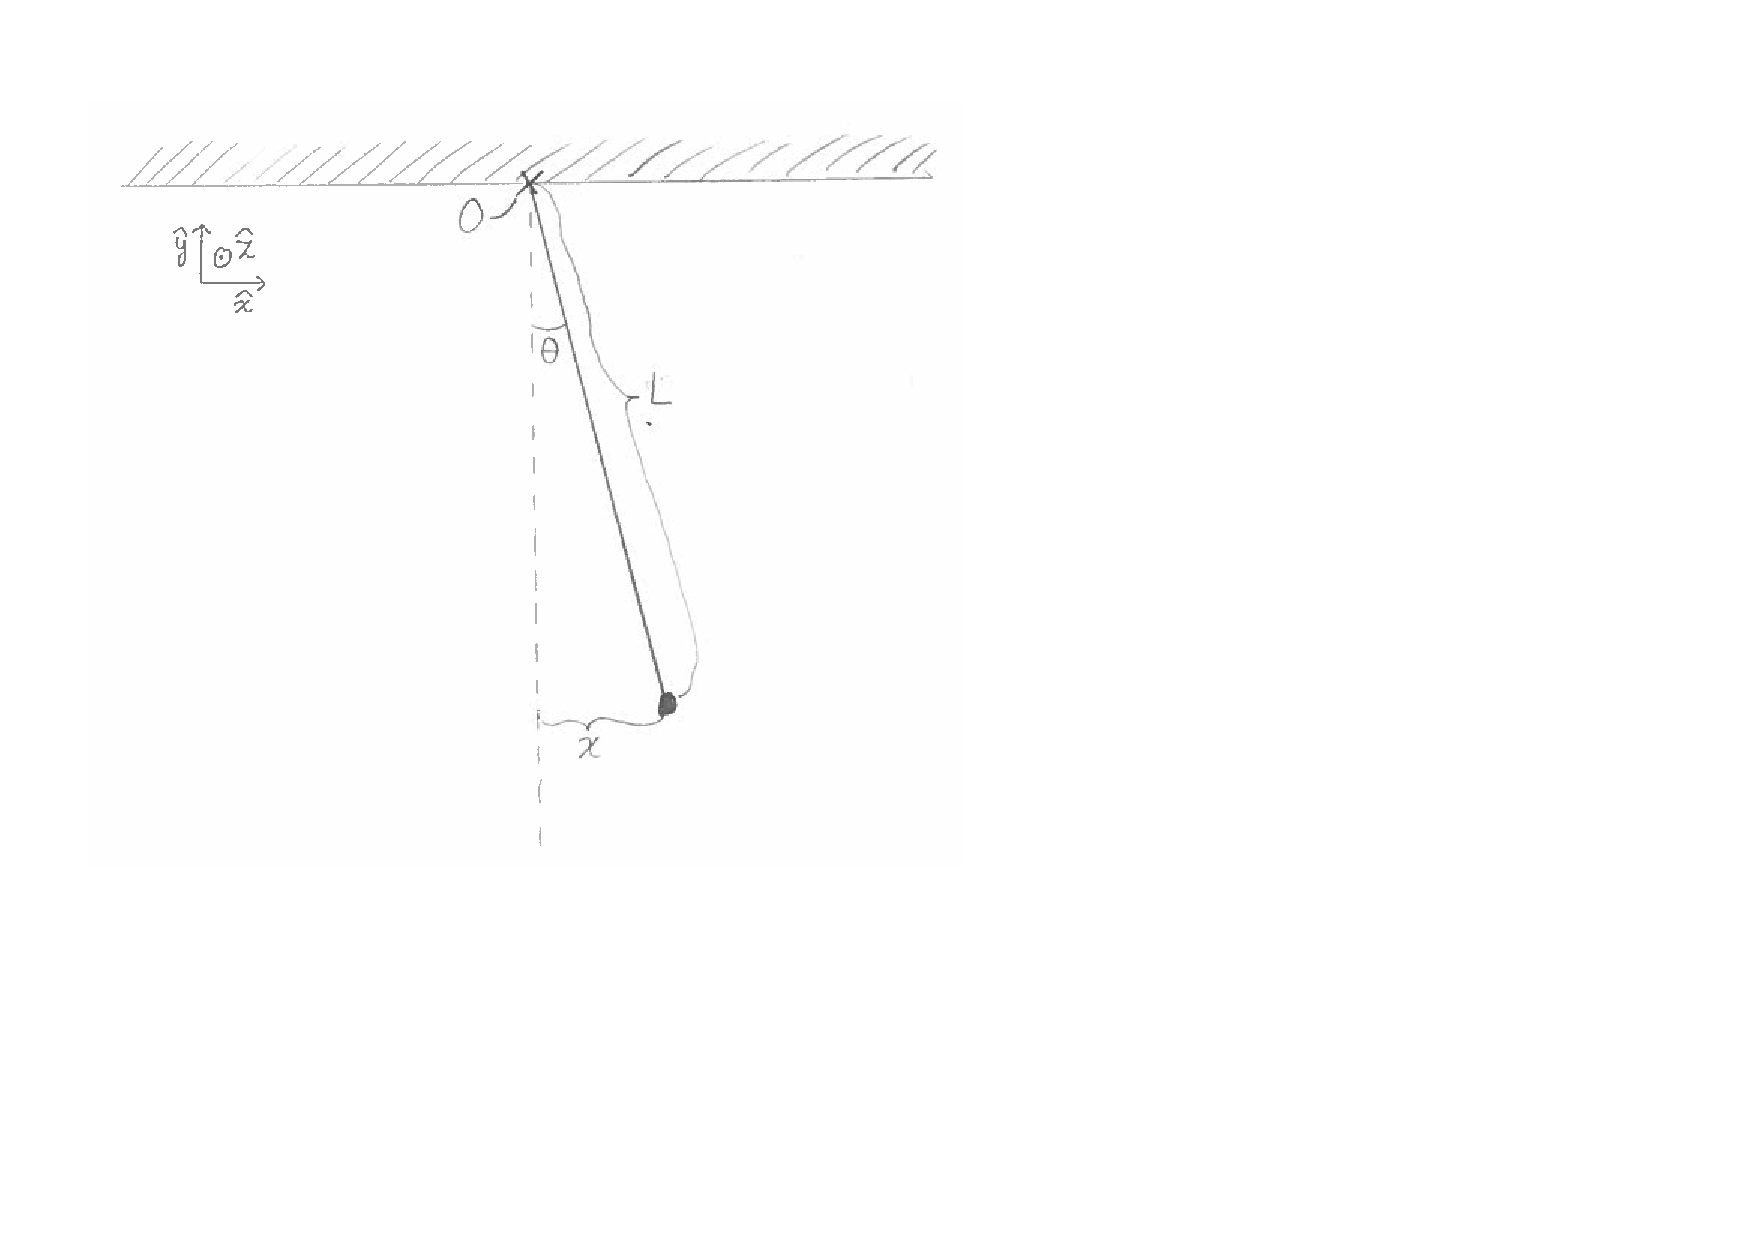
\includegraphics[width=\linewidth]{RotationelMekanik/Pendul}
\caption{Pendul med enhedsvektorer og stedvektor indtegnet til et arbitrært tidspunkt.}
\label{fig:Pendul}
\end{subfigure}
\hspace{5mm}
\begin{subfigure}{.45\textwidth}
  \centering
  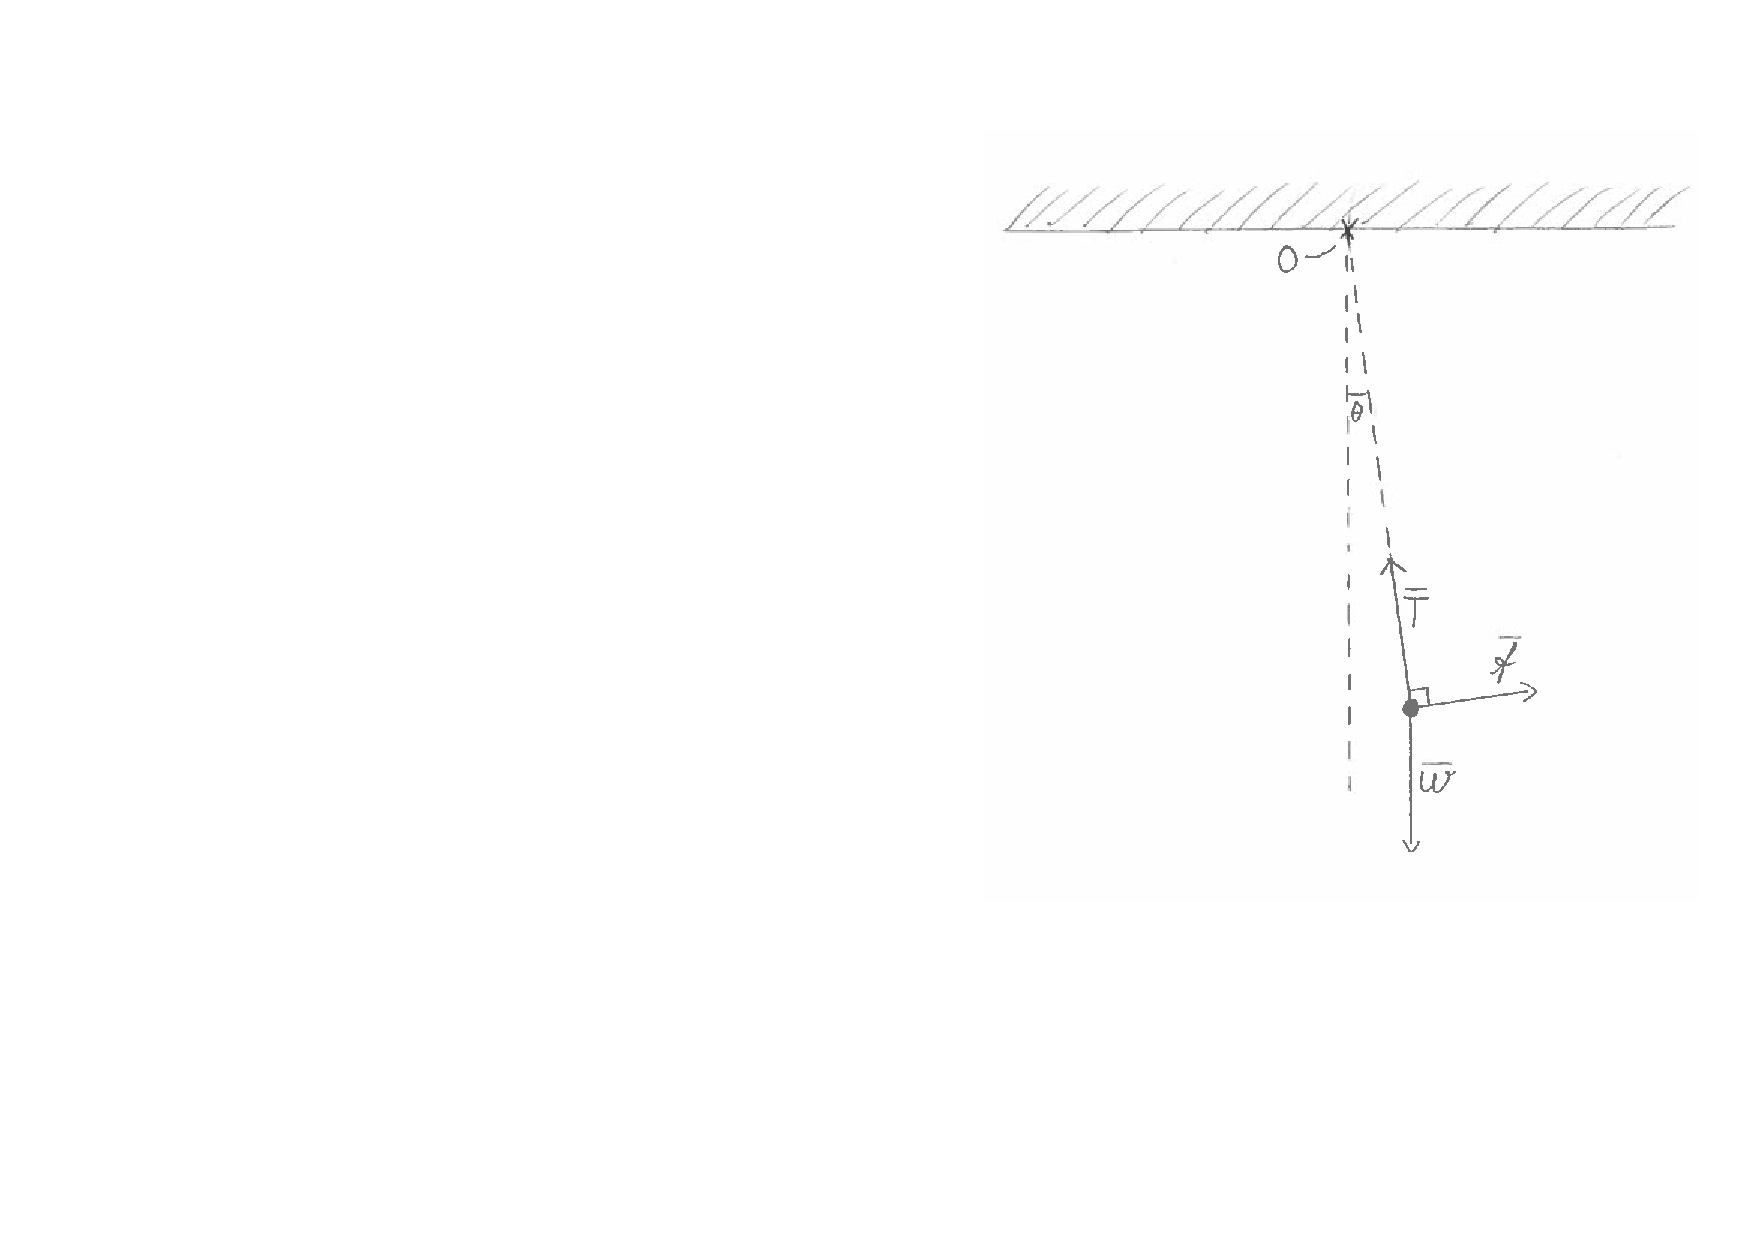
\includegraphics[width=\linewidth]{RotationelMekanik/Kraftanalyse}
  \caption{Kraftanalyse af de på pendulloddet virkende kræfter, der alle antages at have angrebspunkt i massemidtpunktet.}
  \label{fig:Kraftanalyse}
\end{subfigure}
\caption{Tegning af pendulet, der bl.a. viser det valgte koordinatsystem og de virkende kræfter.}
\end{figure}

I første omgang identificeres de på pendullodet virkende kræfter og pendulets ophængningspunkt defineres som origo, se figurene \ref{fig:Pendul} og \ref{fig:Kraftanalyse}. Pendullodets position beskrives ved en retningsvektor $\v{r}$, der går fra ophængningspunktet til lodet. Der er en tyngdekraft, $\v{w}$, en snorkraft, $\v{T}$, og en friktionskraft, $\v{f}$. Tyngdekraften virker til alle tider, $t$, i negativ $y$-retning og skrives derfor som
\begin{align*}
\v{w} = -mg\yhat
\end{align*}
hvor $g$ er tyngdeaccelerationen, og $\yhat$ er en enhedsvektor i $y$-retningen. Defineres $\boldsymbol{\hat{\textbf{r}}}$ som en enhedsvektor parallelt med pendulets retningsvektor, kan snorkraften beskrives som
\begin{align*}
\v{T} = -T\boldsymbol{\hat{\textbf{r}}}
\end{align*}
hvor $T$ er størrelsen på snorkraften. Friktionskraften virker antiparallelt med pendulets hastighed, $\v{v}$, hvorfor den kan beskrives med en skalering $b$ som
\begin{align*}
\v{f} = -b\v{v}
\end{align*}
Idet snoren antages masseløs kan pendulet beskrives som et lod med masse, $m$, der roterer omkring ophængningspunktet, og har ved denne rotation inertimomentet $I$. Snorens længde kaldes $L$ og alle kræfter antages at virke på loddets massemidtpunkt, hvorfor alle kræfters arm kan beskrives som
\begin{align*}
\v{r} = L\boldsymbol{\hat{\textbf{r}}}
\end{align*}
hvilket også et pendulloddets stedvektor. Nu kan kraftmomentet for alle de virkende kræfter bestemmes idet $\v{r}\perp\v{v}\enspace\forall t$
\begin{align*}
\gv{\tau}_w &= \v{r} \times \v{w} = -mgL \cdot \boldsymbol{\hat{\textbf{r}}} \times \yhat = -mgL\sin(\theta)\zhat \\
\gv{\tau}_f &= \v{r} \times \v{f} = -bL \cdot \boldsymbol{\hat{\textbf{r}}} \times \v{v} = -bLv\zhat = -bL^2\d{\theta}{t}\zhat \\
\gv{\tau}_T &= \v{r} \times \v{T} = -TL \cdot \boldsymbol{\hat{\textbf{r}}} \times \v{r} = \v{0}
\end{align*}
hvor subscriptet indikerer hvilken kraft, der behandles. Det samlede kraftmoment bliver derved
\begin{align*}
\sum\gv{\tau} = -\zhat\left(bL^2\d{\theta}{t} + mgL\sin\theta\right)
\end{align*}
Antages pendulets usvingsvinkel at være lille bliver det samlede kraftmomentets størrelse
\begin{align*}
\sum\tau \approx -\left(bL^2\d{\theta}{t} + mgL\theta\right)
\end{align*}
hvor Newtons anden lov for rotationel bevægelse giver differentialligningen
\begin{align*}
\dd{\theta}{t} = -\frac{1}{I}\left(bL^2\d{\theta}{t} + mgL\theta\right)
\end{align*}
som har løsningen
\begin{align*}
\theta(t) = A\exp\left(-\frac{bL^2}{2I}t\right)\cos\left(\omega t + \phi\right), \qquad \omega = \sqrt{\frac{mgL}{I} - \frac{b^2L^4}{4I^2}}
\end{align*}
hvilket medfører at pendulets periode bliver
\begin{align*}
T = \frac{2\pi}{\omega} = 2\pi\left(\frac{mgL}{I} - \frac{b^2L^4}{4I^2}\right)^{-1/2}
\end{align*}
Slutteligt kan pendulets $x$-koordinat beskrives som
\begin{align*}
x(t) = L\sin\theta(t) \approx L\theta(t)
\end{align*}

\subsection*{Simplificerende antagelser}
\subsubsection*{Matematisk pendul med friktion}
Antages lodet at være en punktmasse bliver dets inertimoment
\begin{align*}
I = mL^2
\end{align*}
hvorved  bevægelsesligningen bliver
\begin{align*}
\theta(t) = A\exp\left(-\frac{b}{2m}t\right)\cos\left(\omega t + \phi\right), \qquad \omega = \sqrt{\frac{g}{L} - \frac{b^2}{4m^2}}
\end{align*}
og perioden bliver nu
\begin{align*}
T = \frac{2\pi}{\omega} = 2\pi\left(\frac{g}{L} - \frac{b^2}{4m^2}\right)^{-1/2}
\end{align*}

\subsubsection*{Fysisk pendul uden friktion}
Negligeres friktionen bliver differentialligningen noget simplere, idet pendulet nu vil være i simpel harmonisk bevægelse
\begin{align*}
\dd{\theta}{t} = -\frac{mgL}{I}\theta
\end{align*}
som giver bevægelsesligningen
\begin{align*}
\theta(t) = A\cos\left(\omega t + \phi\right), \qquad \omega = \sqrt{\frac{mgL}{I}}
\end{align*}
og således bliver pendulets periode
\begin{align*}
T = \frac{2\pi}{\omega} = 2\pi\sqrt{\frac{I}{mgL}}
\end{align*}

\subsubsection*{Matematisk pendul uden friktion}
Negligeres friktion og antages pendulets masse at befinde sig i ét punkt kan intertimomentet sættes til $I=mL^2$ i ligningerne fra det fysiske pendul uden friktion
\begin{align*}
\theta(t) = A\cos\left(\omega t + \phi\right), \qquad \omega = \sqrt{\frac{g}{L}}
\end{align*}
hvilket giver en periode på
\begin{align*}
T = \frac{2\pi}{\omega} = 2\pi\sqrt{\frac{L}{g}}
\end{align*}